\section{Electrical}

\subsection{Power Distribution}
The ASV is powered by two 12.8V 8Ah LiFePO4 batteries connected in parallel. A \SI{100}{\watt} solar panel mounted above the electronics enclosure outputs power to an MPPT controller, which continuously regulates the voltage and current to maximize the power output from the solar panel. The charge controller adjusts the variable DC that comes in from the solar panel to a constant voltage and current that is suitable for charging the batteries. The MPPT controller outputs the current through Anderson Powerpole connectors, which are tied into the circuit via a 12p junction terminal block, which distributes power to the rest of the system. The use of Anderson connectors allows for easy connection and disconnection of the solar panel. The batteries are connected with F2 spade connectors, also allowing for easy connection and disconnection. Refer to Figure~\ref{fig:Power_Diagram} for a schematic of the power distribution circuit. The SpeedyBee is shown in Figure~\ref{fig:Speedybee} and the voltage regulator is shown in Figure~\ref{fig:Voltage Regulator}.

\begin{figure}[H]
    \centering
    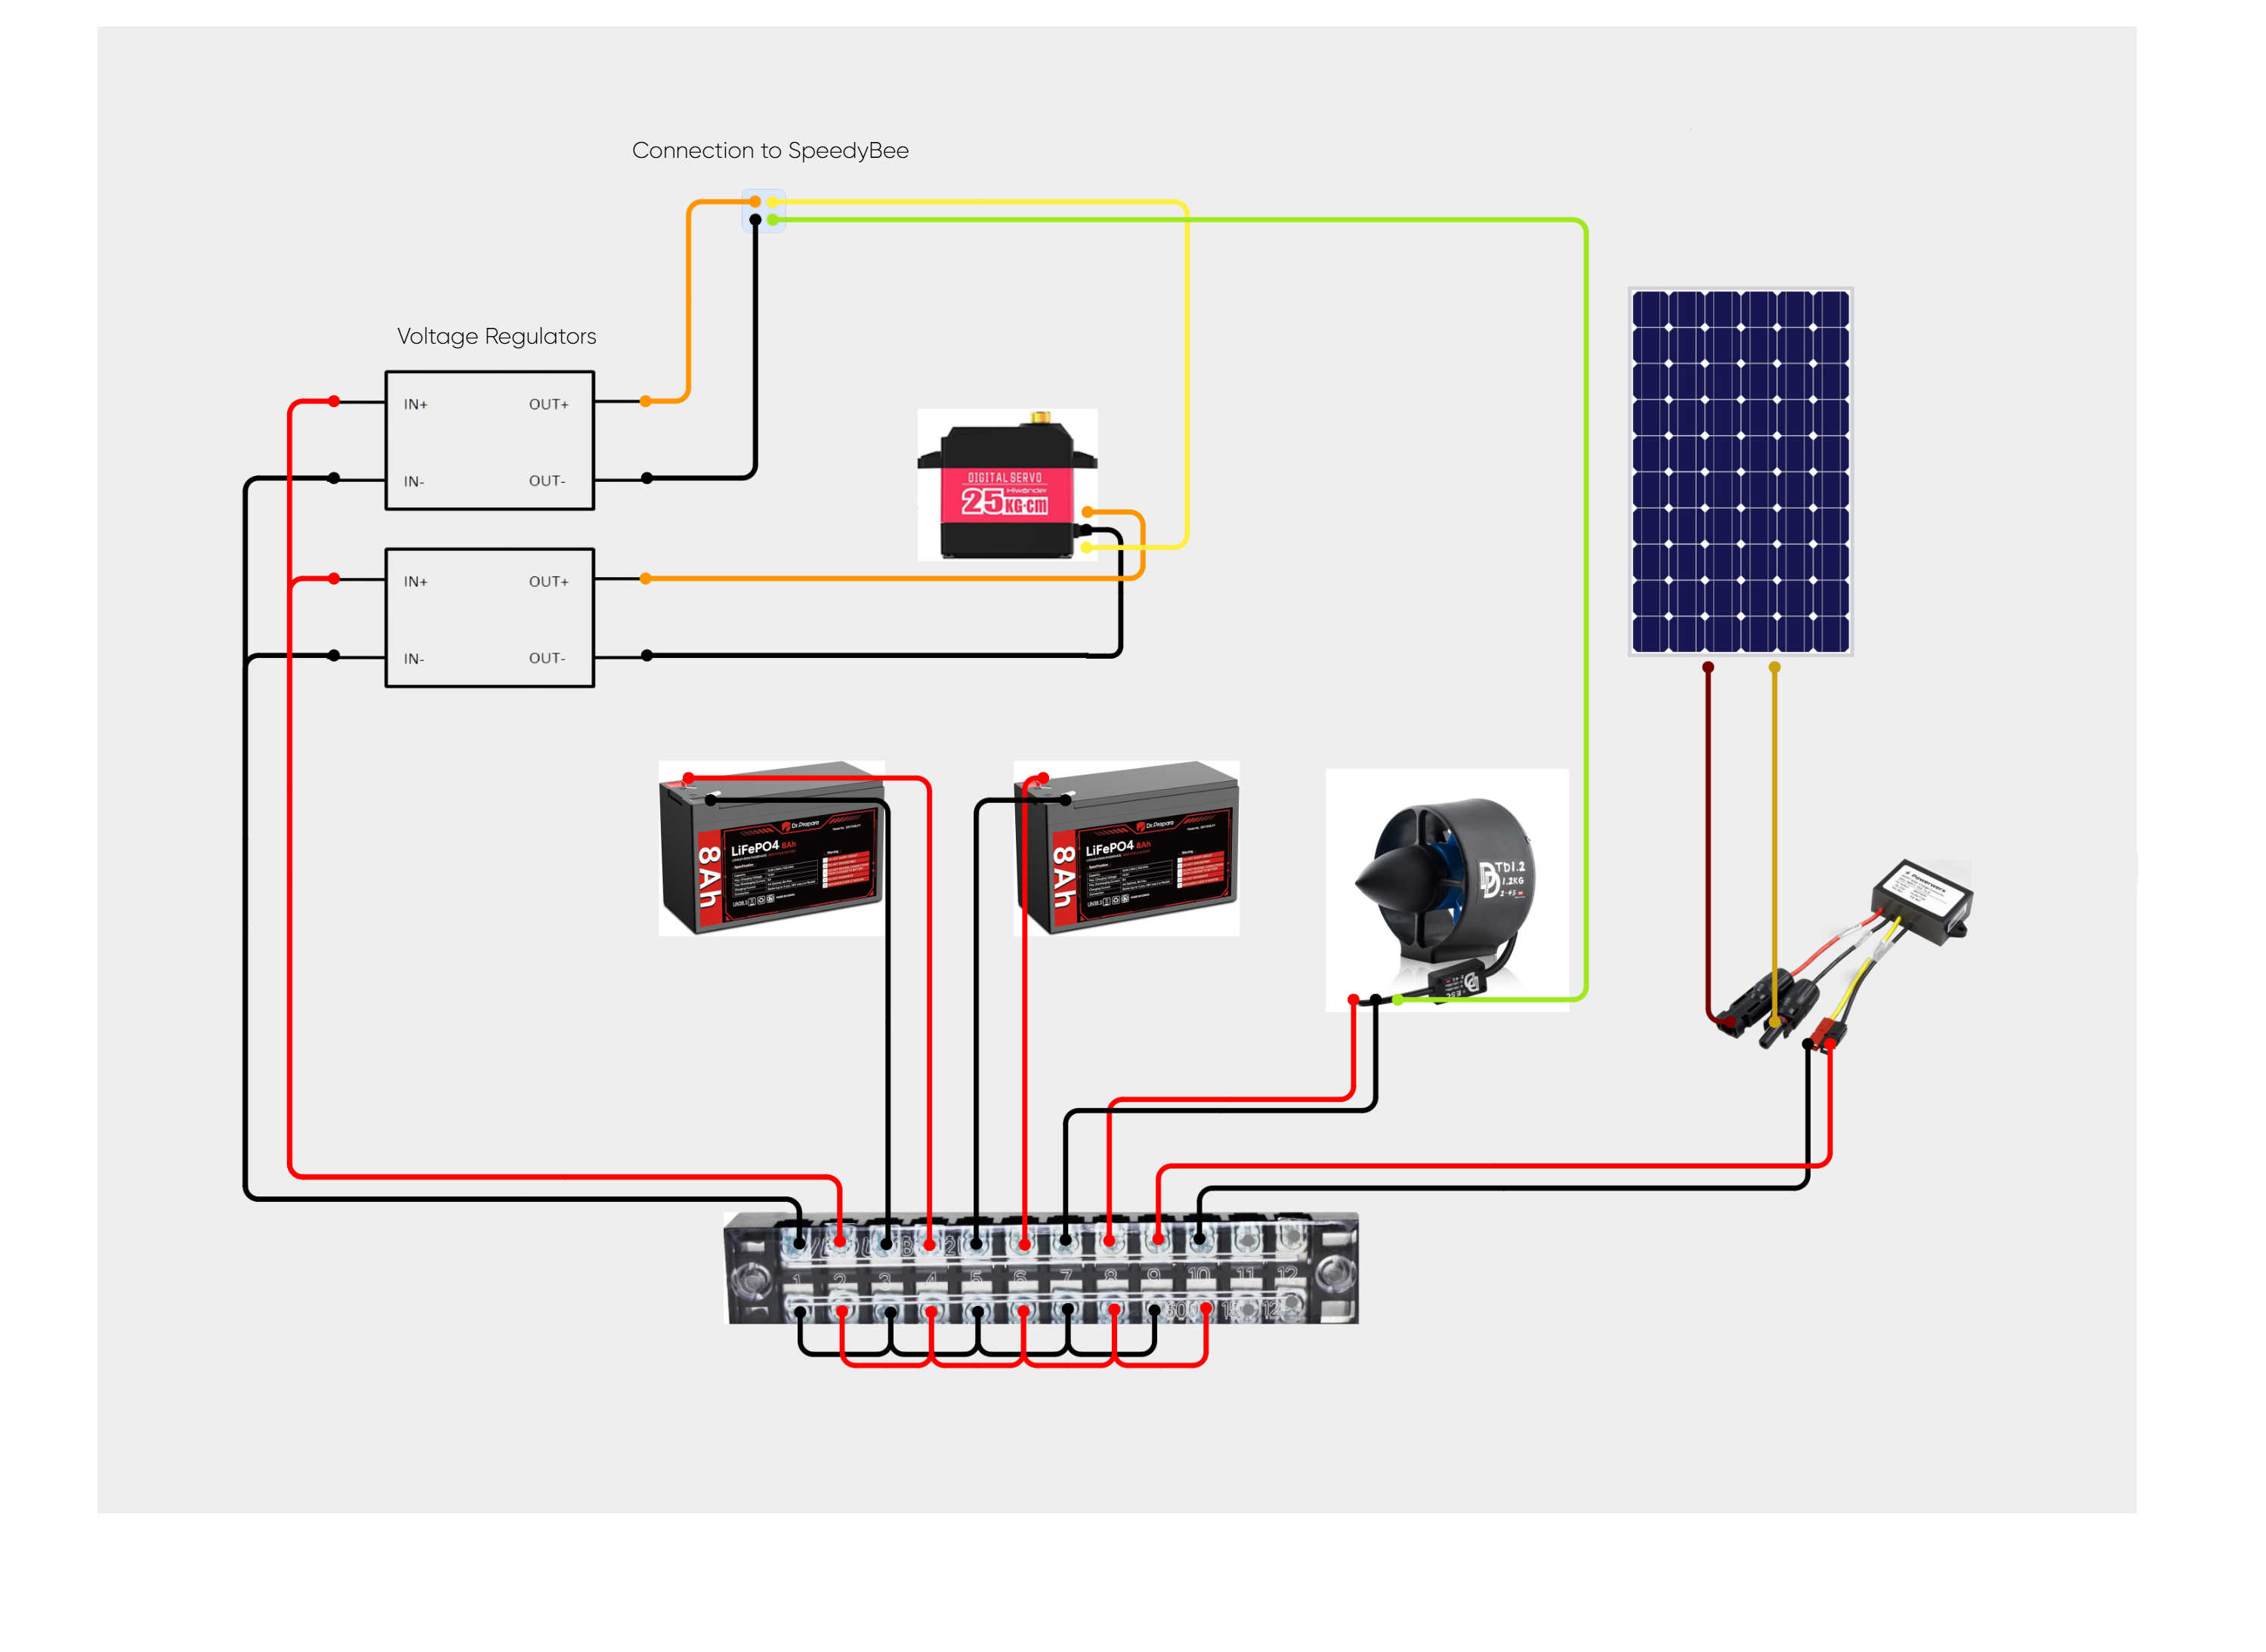
\includegraphics[height=10cm]{Power_Diagram.png}
    \caption{Power Distribution Circuit}
    \label{fig:Power_Diagram}
\end{figure}

Power is distributed through two voltage regulators that step the 12.8V battery voltage down to 5V. One converter supplies the SpeedyBee F405 V4 flight controller and GPS, and the other is dedicated to the servo motor. All components are placed inside a waterproof enclosure with velcro strips. Initially, the voltage regulator was a buck converter on a PCB, but was replaced with a voltage regulator on a protoboard. The buck converter was not able to handle the current draw of the Speedybee, which caused it to overheat and fail. 

\subsubsection{DC-DC Converter and Voltage Regulator}
The PCB design of the buck converter was based primarily on the datasheet recommendations for the TPS563200, targeting an output voltage range of 5–7.5V. See Figure~\ref{fig:DC-DC Converter} capacitors C5, C6, and C7 should all add up to have around 66~\(\mu\)F of output capacitance. the inductor is 3.3~\(\mu\)H and is the recommendation for the output voltage 5-7.5V. This DC-DC converter can provide 3A of current and has an input voltage range of 4.5V to 17V. Future design should include a copper pour between the inductor and output capacitors for heat dissipation, and if more current is needed, consider upgrading to a different chip. However, in our oscilloscope testing, we found that the servo never pulled more than around 0.75A when being held. 

The Voltage Regulator (See Figure~\ref{fig:Voltage Regulator}) provided us a quick and easy solution to the PCB board failures we were having with the DC-DC converters, the L7805CV regulator allowed us to bring 12v down to 5V but didn't allow us to increase or decrease the output voltage with a feedback pin. However, the servo was able to operate with a 5V power and the SpeedyBee was able to power on with 5V as well. The max output current we could output with this chip was internally limited to 1.5A, and if held at max output current for too long, you could deal with some overheating. To fix this, a heat sink could be added, but since we are using the voltage regulator to power our servo, we have never had an issue with overheating.

\subsection{Flight Controller and GPS}
\begin{figure}[H]
    \centering
    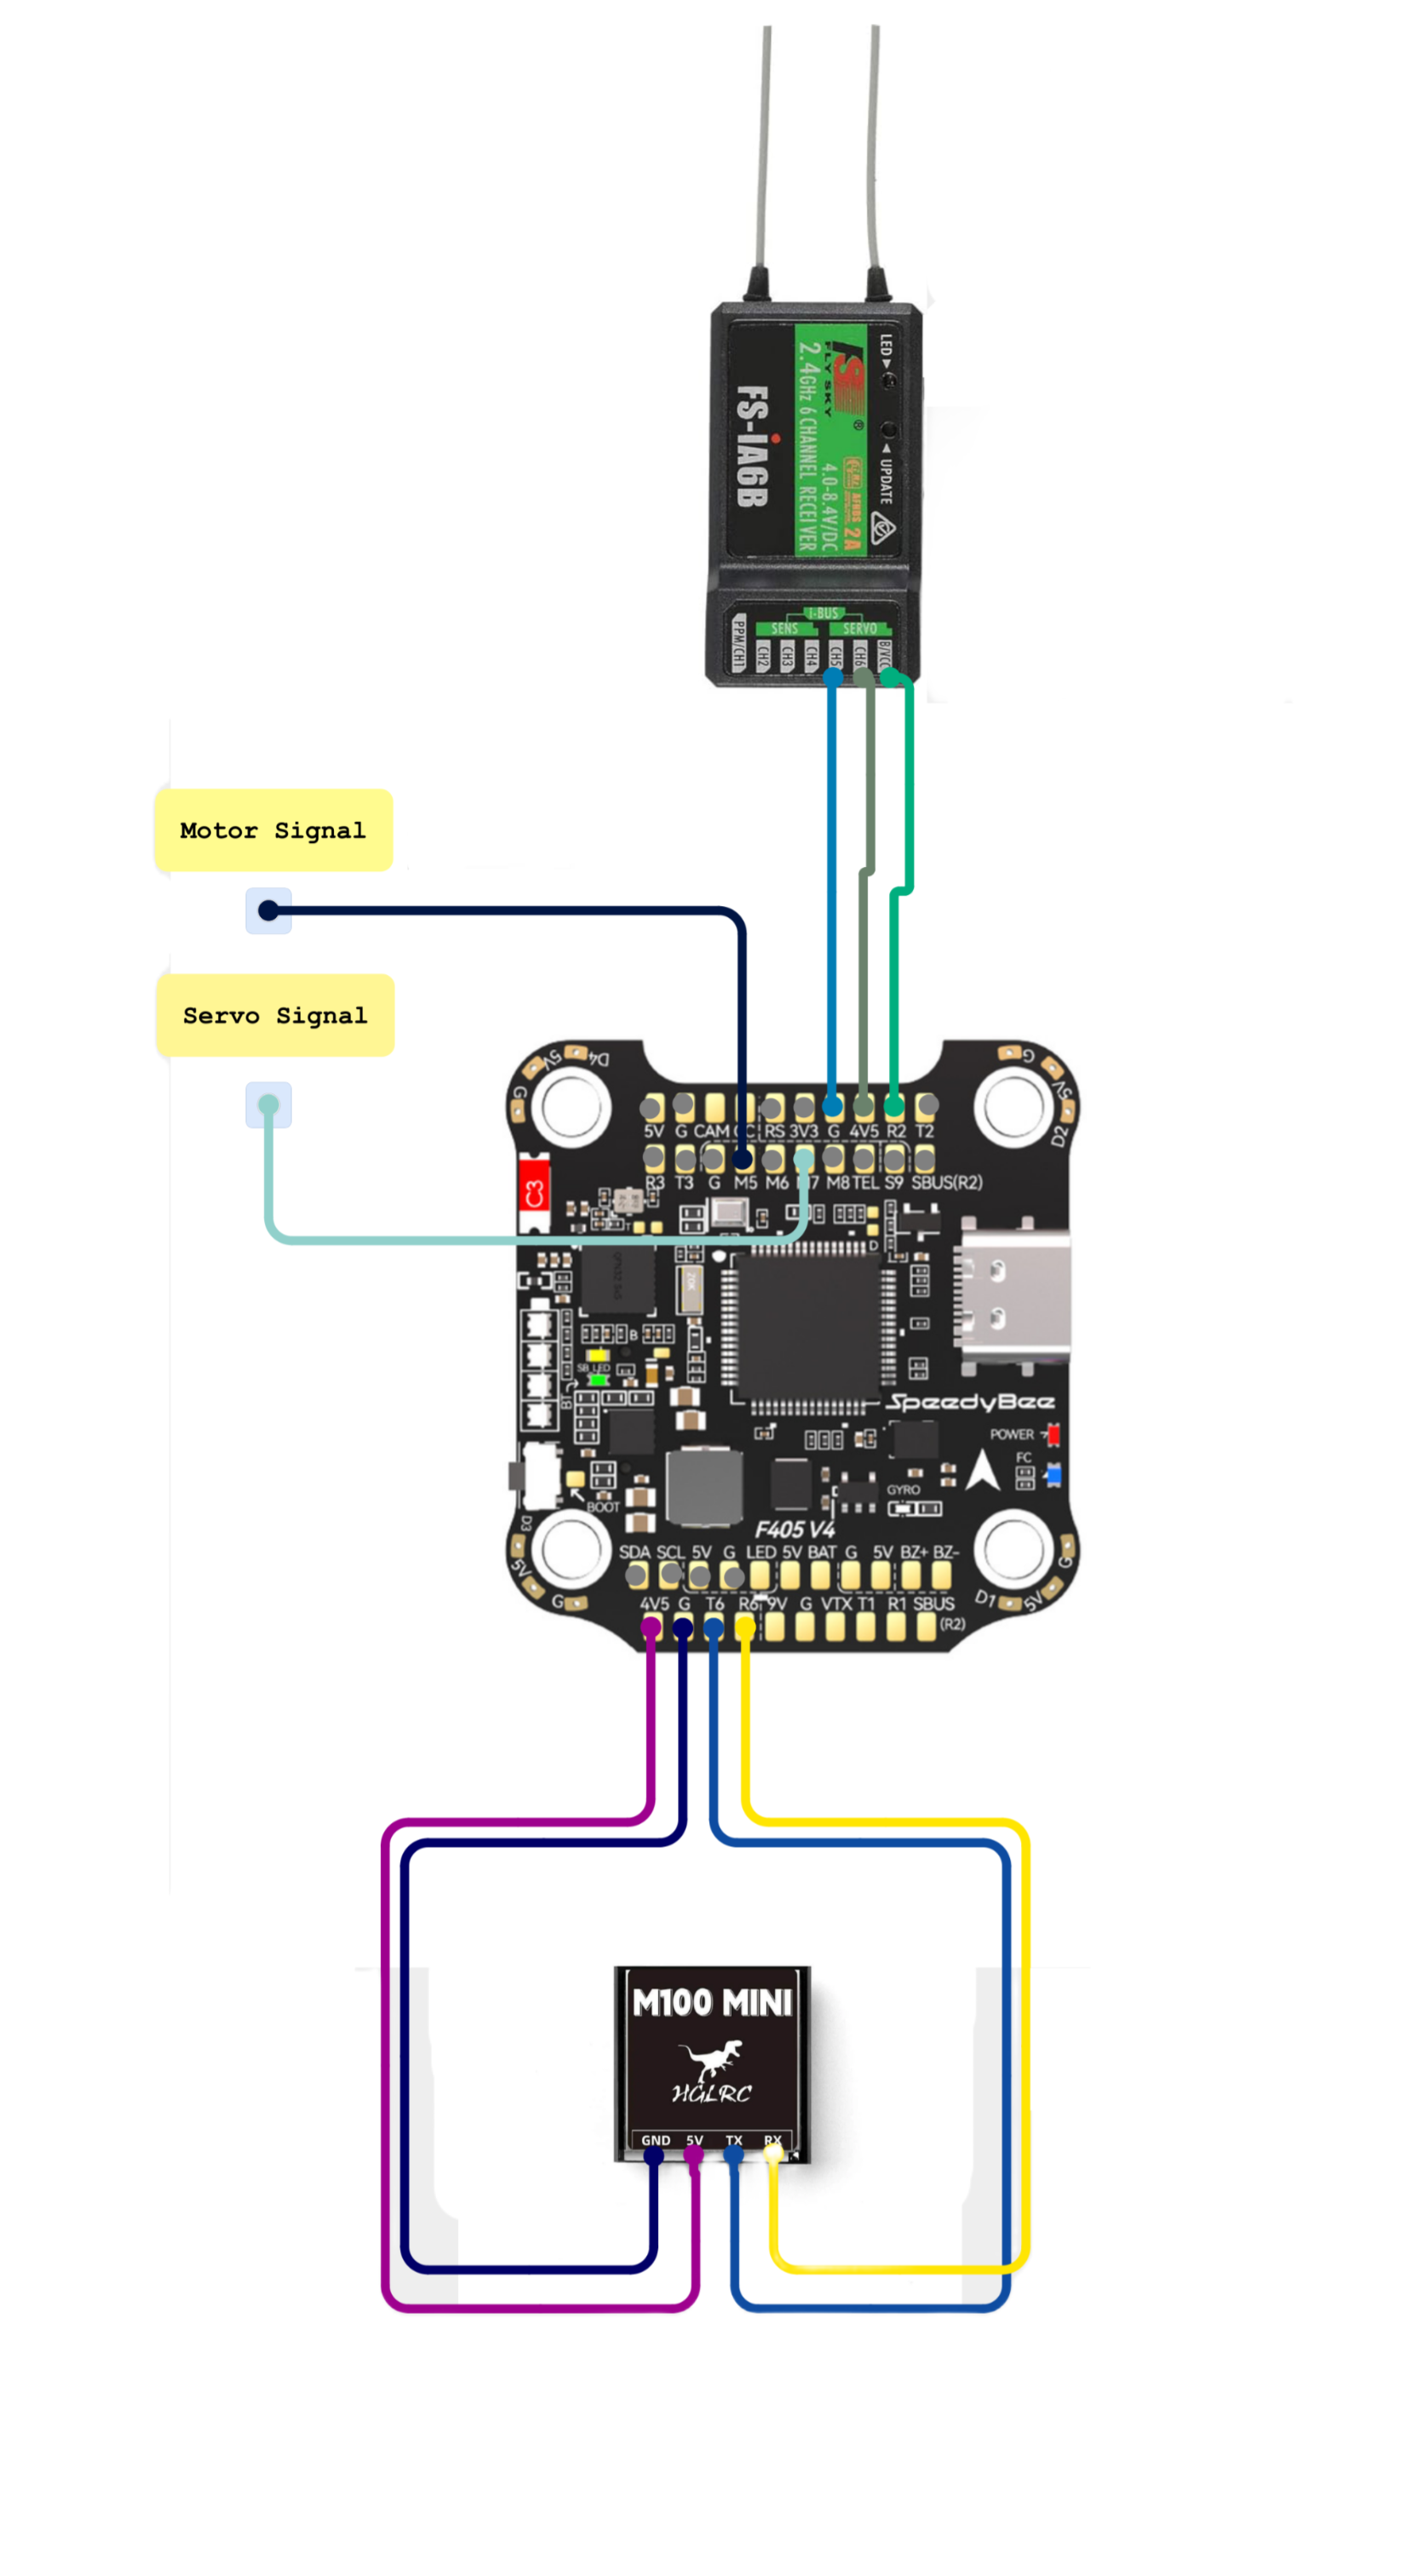
\includegraphics[height=10cm]{speedybee.png}
    \caption{Schematic of the SpeedyBee F405 V4 flight controller and its connections.}
    \label{fig:Speedybee}
\end{figure}

The SpeedyBee F405 V4 flight controller runs iNav firmware and handles both GPS waypoint navigation and motor control. It outputs PWM signals to the brushed DC motor and rudder servo and receives location data from a GPS module. The GPS is soldered directly to UART6 on the flight controller: TX from the GPS is connected to RX6, and RX from the GPS is connected to TX6. A FlySky FS-iA6B receiver is soldered directly to the RX2 pad on the flight controller for SBUS communication, enabling manual RC override when needed.

To generate a magnetic field, a 40 Hz sine wave is created by a prebuilt signal generator and passed through a power amplifier. The amplified signal drives a large copper coil wrapped around the boat’s structure, producing a low-frequency magnetic field detectable by submerged sensors.

The magnetic field \( B \) at the center of a circular coil is given by:

\begin{equation}
B = \frac{\mu_0 N I}{2\pi R}
\label{eq:bfield}
\end{equation}

where:
\begin{itemize}
    \item \( \mu_0 = 4\pi \times 10^{-7} \, \text{T}\cdot\text{m/A} \) is the permeability of free space,
    \item \( N \) is the number of turns in the coil,
    \item \( I \) is the current through the coil,
    \item \( R \) is the radius of the coil.
\end{itemize}

This equation demonstrates that the magnetic field strength increases with more turns or higher current and decreases with a larger coil radius. The 40 Hz frequency was chosen to ensure good penetration through water with minimal signal loss, making it suitable for detection by submerged sensors.

All electrical connections are made using soldered wires. Power and signal lines are routed manually inside the enclosure. Signal and high-current paths are physically separated to minimize noise. Fuses are installed on the battery output lines to protect critical components from short circuits.

The electrical system is simple, modular, and designed for ease of repair and future upgrades. Components can be swapped or rewired without requiring full system disassembly.
\subsection{Signal Generator and Amplifier Boards}
An issue we ran into when trying to provide ample power to our coil to create our desired magnetic moment was how we were going to produce our sine wave. Initially, we wanted to create a sine wave with a modified PWM pin on the Raspberry Pi. However, the output ended up being incredibly noisy and, even after filtering, wasn't super clean. After that solution didn't work, we tried the audio jack, which didn't work for similar reasons, and finally, we tried a DAC, but the noise level was at the same amplitude we wanted to produce our sine wave at. With little time left, we found the best solution was to purchase a signal generator board, and then send the low-frequency sine wave through a power amplifier that could bump up the sine wave to a larger amplitude. This allowed for out-of-the-box options we knew would work and at a cheap cost. However, since this was a last-minute solution, we never fully tested the capabilities of the Signal generator in conjunction with the power amplifier, but this is a brief overview of what we would expect the working solution to look like.
\begin{figure}[H]
    \centering
    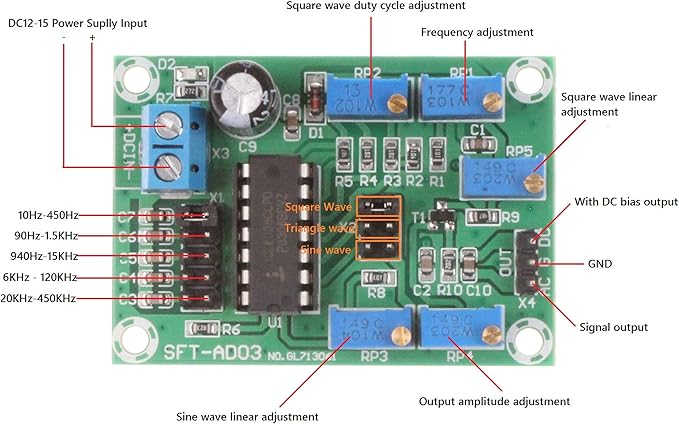
\includegraphics[height=8cm]{Signal Generator.jpg}
    \caption{Signal Generator Overview}
    \label{fig:Signal Generator}
\end{figure}
Fig. \ref{fig:Signal Generator} gives us a nice overview of what the signal generator PCB can do. The main chip used in this board is the ICL8038, which can take in 10 - 30V and can output a sine wave, a square wave, and a triangle wave. For our purposes, we will strictly be outputting a Sine wave. With the potentiometers located at the bottom right of the board and the top right of the board, we can control the frequency and amplitude. We can go as low as 10Hz, which is perfect for the low frequency that we need. Due to the limited time frame when we never fully got to test the working condition of this board; however, these normally work straight out of the box, and we can expect a positive output since we are within the working parameters of the ICL8038.

\begin{figure}[H]
    \centering
    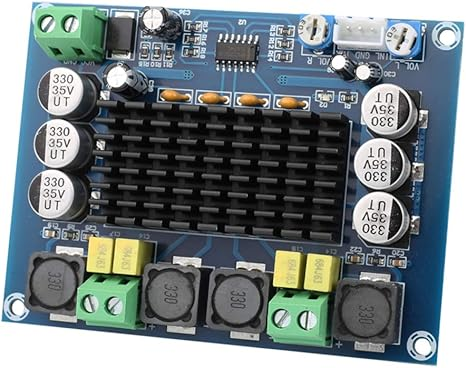
\includegraphics[height=8cm]{power_amp.jpg}
    \caption{Power Amplifier}
    \label{fig:Power Amplifier}
\end{figure}
Fig. \ref{fig:Power Amplifier} shows the Power Amplifier board we bought and used to up a low frequency sine wave up to get our desired current amplitude. looking at the top of the board we can see an input channel and a power channel for 12V DC. the main chip in this board is the TPA3116D2 which has a 